% Options for packages loaded elsewhere
\PassOptionsToPackage{unicode}{hyperref}
\PassOptionsToPackage{hyphens}{url}
\documentclass[
]{article}
\usepackage{xcolor}
\usepackage{amsmath,amssymb}
\setcounter{secnumdepth}{-\maxdimen} % remove section numbering
\usepackage{iftex}
\ifPDFTeX
  \usepackage[T1]{fontenc}
  \usepackage[utf8]{inputenc}
  \usepackage{textcomp} % provide euro and other symbols
\else % if luatex or xetex
  \usepackage{unicode-math} % this also loads fontspec
  \defaultfontfeatures{Scale=MatchLowercase}
  \defaultfontfeatures[\rmfamily]{Ligatures=TeX,Scale=1}
\fi
\usepackage{lmodern}
\ifPDFTeX\else
  % xetex/luatex font selection
\fi
% Use upquote if available, for straight quotes in verbatim environments
\IfFileExists{upquote.sty}{\usepackage{upquote}}{}
\IfFileExists{microtype.sty}{% use microtype if available
  \usepackage[]{microtype}
  \UseMicrotypeSet[protrusion]{basicmath} % disable protrusion for tt fonts
}{}
\makeatletter
\@ifundefined{KOMAClassName}{% if non-KOMA class
  \IfFileExists{parskip.sty}{%
    \usepackage{parskip}
  }{% else
    \setlength{\parindent}{0pt}
    \setlength{\parskip}{6pt plus 2pt minus 1pt}}
}{% if KOMA class
  \KOMAoptions{parskip=half}}
\makeatother
\usepackage{graphicx}
\makeatletter
\newsavebox\pandoc@box
\newcommand*\pandocbounded[1]{% scales image to fit in text height/width
  \sbox\pandoc@box{#1}%
  \Gscale@div\@tempa{\textheight}{\dimexpr\ht\pandoc@box+\dp\pandoc@box\relax}%
  \Gscale@div\@tempb{\linewidth}{\wd\pandoc@box}%
  \ifdim\@tempb\p@<\@tempa\p@\let\@tempa\@tempb\fi% select the smaller of both
  \ifdim\@tempa\p@<\p@\scalebox{\@tempa}{\usebox\pandoc@box}%
  \else\usebox{\pandoc@box}%
  \fi%
}
% Set default figure placement to htbp
\def\fps@figure{htbp}
\makeatother
% definitions for citeproc citations
\NewDocumentCommand\citeproctext{}{}
\NewDocumentCommand\citeproc{mm}{%
  \begingroup\def\citeproctext{#2}\cite{#1}\endgroup}
\makeatletter
 % allow citations to break across lines
 \let\@cite@ofmt\@firstofone
 % avoid brackets around text for \cite:
 \def\@biblabel#1{}
 \def\@cite#1#2{{#1\if@tempswa , #2\fi}}
\makeatother
\newlength{\cslhangindent}
\setlength{\cslhangindent}{1.5em}
\newlength{\csllabelwidth}
\setlength{\csllabelwidth}{3em}
\newenvironment{CSLReferences}[2] % #1 hanging-indent, #2 entry-spacing
 {\begin{list}{}{%
  \setlength{\itemindent}{0pt}
  \setlength{\leftmargin}{0pt}
  \setlength{\parsep}{0pt}
  % turn on hanging indent if param 1 is 1
  \ifodd #1
   \setlength{\leftmargin}{\cslhangindent}
   \setlength{\itemindent}{-1\cslhangindent}
  \fi
  % set entry spacing
  \setlength{\itemsep}{#2\baselineskip}}}
 {\end{list}}
\usepackage{calc}
\newcommand{\CSLBlock}[1]{\hfill\break\parbox[t]{\linewidth}{\strut\ignorespaces#1\strut}}
\newcommand{\CSLLeftMargin}[1]{\parbox[t]{\csllabelwidth}{\strut#1\strut}}
\newcommand{\CSLRightInline}[1]{\parbox[t]{\linewidth - \csllabelwidth}{\strut#1\strut}}
\newcommand{\CSLIndent}[1]{\hspace{\cslhangindent}#1}
\setlength{\emergencystretch}{3em} % prevent overfull lines
\providecommand{\tightlist}{%
  \setlength{\itemsep}{0pt}\setlength{\parskip}{0pt}}
\usepackage{bookmark}
\IfFileExists{xurl.sty}{\usepackage{xurl}}{} % add URL line breaks if available
\urlstyle{same}
\hypersetup{
  pdftitle={TRANSFORMANDO APIS EM INTERFACES CONVERSACIONAIS: VALIDAÇÃO DA ABORDAGEM OPENAPI-MCP PARA AGENTES BASEADOS EM IA},
  hidelinks,
  pdfcreator={LaTeX via pandoc}}

\title{\textbf{TRANSFORMANDO APIS EM INTERFACES CONVERSACIONAIS:
VALIDAÇÃO DA ABORDAGEM OPENAPI-MCP PARA AGENTES BASEADOS EM IA}}
\author{}
\date{}

\begin{document}
\maketitle

\textbf{Lucas de Castro Zanoni}\footnote{Graduando em Engenharia de
  software no semestre letivo de 2025-1. E-mail:
  castro.lucas290@gmail.com}

\textbf{Thyerri Fernandes Mezzari}\footnote{Professor do Centro
  Universitário UniSATC E-mail: thyerri.mezzari@satc.edu.br}

Resumo: Este trabalho apresenta um estudo experimental de integração de
agentes conversacionais baseados em inteligência artificial a soluções
web através da especificação OpenAPI combinada com o protocolo Model
Context Protocol (MCP). A pesquisa investiga como especificações OpenAPI
podem ser automaticamente convertidas em servidores MCP, permitindo que
modelos de linguagem de grande escala (LLMs) interajam de forma
padronizada e segura com sistemas externos. Para garantir uma análise
rigorosa e reprodutível, foi desenvolvida uma interface padronizada e
definidos critérios objetivos, fundamentando-se em referências
acadêmicas, guias de segurança, relatórios de mercado e documentações
oficiais de provedores de modelos de linguagem. O estudo envolveu a
implementação de uma prova de conceito que inclui um gerador automático
de servidores MCP a partir de especificações OpenAPI, um cliente de chat
capaz de gerenciar múltiplos servidores MCP simultaneamente, e
aplicações de teste para validação da abordagem. Foram aplicados testes
automatizados end-to-end, com ênfase em métricas de robustez, segurança
(incluindo red teaming e injeção de prompts) e usabilidade. Os
resultados demonstram a viabilidade e eficácia da integração
OpenAPI-MCP, fornecendo uma análise fundamentada sobre os benefícios,
desafios e limitações desta abordagem para a integração de agentes
conversacionais em sistemas complexos, promovendo acessibilidade,
usabilidade e confiabilidade.

\textbf{Palavras-chave:} agente conversacional, integração de sistemas,
inteligência artificial, OpenAPI, Model Context Protocol, segurança,
usabilidade.

\section{1 INTRODUÇÃO}\label{introduuxe7uxe3o}

A evolução das interfaces de usuário tem gerado uma diversidade de
padrões de design e usabilidade, resultando frequentemente em barreiras
para a plena acessibilidade e interação dos usuários com os sistemas
digitais. Com o aumento da complexidade do frontend e a multiplicidade
de paradigmas de interação, muitos usuários enfrentam dificuldades
significativas para utilizar efetivamente as funcionalidades oferecidas
pelas soluções web modernas (RAPP et al., 2018) (KOCABALLI et al.,
2019). Nesse contexto, a ascensão dos Modelos de Linguagem de Grande
Escala (LLMs), como os desenvolvidos por OpenAI, Anthropic e Google, tem
impulsionado o desenvolvimento de agentes conversacionais mais avançados
e adaptáveis (ANTHROPIC, 2024a; OPENAI, 2022). Nos últimos anos, avanços
em modelos baseados em Transformer, como o BERT (2018), que aprimorou a
compreensão textual, e o GPT-3 (2020), que ampliou as capacidades
generativas e o aprendizado com poucos exemplos (\emph{few-shot}),
permitiram que os LLMs realizassem tarefas cada vez mais complexas a
partir de simples instruções em linguagem natural. Esses avanços
consolidaram os LLMs como interfaces conversacionais robustas e eficazes
para integração com sistemas.

Diante desse cenário, estudos recentes têm demonstrado que agentes
conversacionais podem aprimorar significativamente a experiência do
usuário ao simplificar interações com sistemas complexos (FAST et al.,
2017). Além disso, a implementação de interfaces baseadas em linguagem
natural tem mostrado potencial para melhorar a usabilidade em contextos
domésticos e inteligentes, reduzindo o tempo e o esforço necessários
para completar tarefas complexas (GUO et al., 2024). Ademais, tais
interfaces oferecem vantagens consideráveis em termos de acessibilidade,
permitindo uma comunicação mais inclusiva e adaptável a usuários com
diferentes necessidades especiais (LISTER et al., 2020) (DENG, 2023).
Para que esses benefícios sejam efetivamente alcançados em soluções web,
é fundamental avaliar as diferentes estratégias de integração desses
agentes aos sistemas existentes.

Nesse sentido, este estudo aborda experimentalmente a integração de
agentes conversacionais baseados em IA a sistemas web através da
especificação OpenAPI combinada com o protocolo emergente MCP (Model
Context Protocol). Esta abordagem permite que especificações OpenAPI
sejam automaticamente convertidas em servidores MCP, criando uma ponte
padronizada entre modelos de linguagem e sistemas externos. A solução
será avaliada quanto a desempenho, segurança, facilidade de
implementação e experiência do usuário, com foco específico na
capacidade de gerenciar múltiplos servidores MCP simultaneamente e na
eficácia da geração automática de código.

Dessa forma, a problemática central desta pesquisa reside na questão:
como a combinação da especificação OpenAPI com o protocolo MCP pode
facilitar a integração eficiente e segura de agentes conversacionais
baseados em IA com sistemas web existentes? Essa pergunta reflete a
necessidade crescente de soluções padronizadas que democratizem o acesso
à tecnologia, reduzindo a complexidade de integração e tornando sistemas
especializados mais acessíveis através de interfaces conversacionais
naturais.

A relevância deste estudo evidencia-se pelo potencial transformador que
os agentes conversacionais representam para a área de interação
humano-computador. Ao implementar um sistema intermediário capaz de
interpretar linguagem natural e traduzi-la em ações específicas dentro
de um sistema, cria-se uma ponte que permite aos usuários interagir de
forma mais intuitiva e natural com as tecnologias digitais. Esta
abordagem tem o potencial de mitigar as barreiras impostas por
interfaces complexas, contribuindo para uma maior inclusão digital e
para a melhoria da experiência do usuário em diversos contextos de
aplicação.

\section{2 PROCEDIMENTO EXPERIMENTAL}\label{procedimento-experimental}

Este estudo adota uma abordagem experimental estruturada em etapas
sequenciais para investigar a viabilidade e eficácia da integração de
agentes conversacionais baseados em IA a sistemas web através da
especificação OpenAPI combinada com o protocolo Model Context Protocol
(MCP). A pesquisa será examinada com base em uma prova de conceito
prática, desenvolvida para validar sua viabilidade técnica e avaliar
objetivamente aspectos funcionais e não-funcionais da solução proposta.

Inicialmente, será conduzida uma revisão sistemática da literatura,
consolidando conhecimentos científicos sobre integração OpenAPI-MCP e
embasando teoricamente a fase experimental. Na sequência, a estratégia
será implementada e testada por meio de uma prova de conceito
abrangente, incluindo o desenvolvimento de um gerador automático de
servidores MCP, um cliente de chat para gerenciamento de múltiplos
servidores, e aplicações de teste para validação da abordagem.

Os critérios de avaliação definidos incluem desempenho, segurança,
facilidade de implementação, manutenibilidade e experiência do usuário.
Para assegurar resultados objetivos e reproduzíveis, os testes incluirão
análises automatizadas end-to-end, medidas de robustez e segurança (como
testes de red teaming e proteção contra injeção de prompts) e avaliações
qualitativas de usabilidade. Os resultados serão sistematicamente
documentados e analisados, permitindo identificar desafios, vantagens e
limitações intrínsecas à integração OpenAPI-MCP e demonstrando sua
aplicabilidade prática para diferentes contextos de uso.

\subsection{2.1 MATERIAIS}\label{materiais}

Para garantir a rigorosidade científica e a reprodutibilidade dos
experimentos conduzidos neste estudo, é essencial uma seleção criteriosa
dos materiais e ferramentas utilizados. Esta seção detalha os recursos
específicos empregados na condução desta pesquisa, justificando sua
escolha baseada na eficiência, popularidade, robustez e aplicabilidade
prática dentro do contexto dos agentes conversacionais e integração de
sistemas.

\subsubsection{2.1.1 NODE.JS PARA DESENVOLVIMENTO DAS PROVAS DE
CONCEITO}\label{node.js-para-desenvolvimento-das-provas-de-conceito}

Node.js foi escolhido como plataforma principal para o desenvolvimento
das provas de conceito devido à sua comprovada eficácia na integração de
sistemas baseados em inteligência artificial (IA), especialmente com
agentes conversacionais e LLMs. A plataforma é amplamente adotada devido
à sua arquitetura orientada a eventos e capacidade de gerenciar
eficientemente múltiplas conexões simultâneas, essencial para aplicações
que exigem respostas rápidas em tempo real (CHEREDNICHENKO et al.,
2024).

Relatórios da \emph{Red Hat} destacam que o uso eficiente da arquitetura
assíncrona do Node.js possibilita a criação de agentes baseados em LLMs
com alta performance e escalabilidade. Isso garante um gerenciamento
eficiente de múltiplas operações paralelas, essencial para aplicações
intensivas em IA e integração com APIs externas (BLOG, 2024).

\subsubsection{\texorpdfstring{2.1.2 TESTES \emph{END-TO-END}
(E2E)}{2.1.2 TESTES END-TO-END (E2E)}}\label{testes-end-to-end-e2e}

O \emph{Framework} de Gerenciamento de Riscos de IA do NIST (OPREA;
VASSILEV, 2023) destaca a importância de avaliar o desempenho de
sistemas de IA de forma abrangente, defendendo que testes de integração
devem avaliar os sistemas de ponta a ponta para identificar erros de
integração e garantir a precisão das respostas em cenários realistas.
Testes rigorosos como esses não apenas identificam problemas de
integração, mas também asseguram às partes interessadas que o sistema se
comporta conforme o esperado em condições do mundo real.

A injeção de \emph{prompt} representa um risco significativo em
implantações de LLMs em nosso cenário, no qual o modelo possui acesso a
dados e sistemas potencialmente críticos, incluindo, ocasionalmente,
conexões diretas com dados brutos de banco de dados. O guia de riscos da
OWASP (JOHN et al., 2025) classifica a injeção de \emph{prompt} como uma
ameaça crítica à segurança, destacando a necessidade de procedimentos de
teste rigorosos para garantir que agentes conversacionais baseados em
LLMs não revelem inadvertidamente dados sensíveis ou contornem
restrições do sistema quando expostos a entradas maliciosas.
Recentemente, Wu et al.~(2023) (WU et al., 2023) demonstraram que
ataques de \emph{jailbreak} --- um tipo avançado de injeção de
\emph{prompt} --- podem burlar as salvaguardas éticas de modelos como o
ChatGPT em até 67\% dos casos, gerando conteúdos prejudiciais como
extorsão e desinformação.

Com isso em mente, o uso de testes E2E pode ser utilizado para avaliar a
resiliência da implementação ao simular entradas adversárias, processo
conhecido como \emph{red teaming}. Segundo Inie et al.~(2025) (INIE;
STRAY; DERCZYNSKI, 2025), o \emph{red teaming} desafia sistematicamente
sistemas de IA com \emph{prompts} adversários projetados para testar
seus limites e mecanismos de segurança. Ao encapsular consultas do
usuário com lembretes de responsabilidade ética (e.g., ``Você deve ser
um ChatGPT responsável''), o método reduziu a taxa de sucesso de
\emph{jailbreaks} para 19\%, mantendo a funcionalidade padrão do modelo
--- um resultado validado através de testes E2E em 540 cenários
adversarialmente projetados (WU et al., 2023).

\subsubsection{2.1.3 MODELOS DE LINGUAGEM DE GRANDE ESCALA
(LLMs)}\label{modelos-de-linguagem-de-grande-escala-llms}

Os LLMs, incluindo tecnologias como OpenAI GPT, Anthropic e modelos
disponibilizados pela Google, são essenciais neste estudo devido à sua
capacidade de interpretar e gerar linguagem natural de forma avançada e
eficaz. Estes modelos foram selecionados por sua performance comprovada
e ampla adoção em pesquisas acadêmicas e no mercado corporativo,
proporcionando um sólido embasamento para as funcionalidades de
interação do agente conversacional.

\paragraph{2.1.3.1 HISTÓRICO DO DESENVOLVIMENTO DE LLMS
(2018--2023)}\label{histuxf3rico-do-desenvolvimento-de-llms-20182023}

Nos últimos cinco anos, os LLMs evoluíram rapidamente, a partir da
arquitetura Transformer. O lançamento do BERT (2018) mostrou avanços em
compreensão textual, enquanto a série GPT demonstrou fortes capacidades
generativas. O GPT-3 (2020), com 175 bilhões de parâmetros, evidenciou
habilidades emergentes de aprendizado com poucos exemplos
(\emph{few-shot}), ampliando o escopo de tarefas possíveis por meio de
simples instruções em linguagem natural (BROWN et al., 2020).

A partir de 2022, o foco da pesquisa passou a ser o aprimoramento do
raciocínio e alinhamento dos LLMs. Técnicas como \emph{Chain-of-Thought
prompting} permitiram que os modelos resolvessem problemas complexos de
forma mais eficaz (WEI et al., 2023). O uso de Reinforcement Learning
from Human Feedback (RLHF), como nos modelos InstructGPT e
posteriormente ChatGPT, melhorou a capacidade dos LLMs de seguir
instruções com mais segurança e consistência. Esses avanços
estabeleceram as bases para o uso dos LLMs como interfaces
conversacionais robustas em cenários de integração com sistemas (OPENAI,
2022).

\paragraph{2.1.3.2 EXTENSÃO DE JANELA DE
CONTEXTO}\label{extensuxe3o-de-janela-de-contexto}

Com o avanço dos modelos, observou-se uma tendência significativa no
aumento das janelas de contexto --- a quantidade de tokens que um LLM
pode processar em uma única interação. Modelos como o Claude 3 já
alcançam até 100.000 tokens (ANTHROPIC, 2024b), enquanto versões
estendidas do GPT-4 suportam até 32.000 tokens (OPENAI, 2023a). Esse
aumento permite que os modelos processem documentos extensos, múltiplas
conversas ou grandes volumes de dados em uma única solicitação,
superando, em muitos casos, abordagens tradicionais baseadas em
retrieval-augmented generation (RAG), especialmente em tarefas que
exigem síntese contextual profunda.

A capacidade de manter longos contextos é altamente benéfica para
integração com sistemas -- um LLM pode manter diálogos prolongados,
lembrar estados extensos ou ingerir bancos de dados e logs inteiros de
uma só vez. No entanto, isso traz custos computacionais consideráveis, e
há esforços contínuos para utilizar essas janelas maiores de forma
eficiente (por exemplo, condensando ou focando a atenção nas partes mais
relevantes) (ANTHROPIC, 2024b; OPENAI, 2023a).

\paragraph{2.1.3.3 RACIOCÍNIO APRIMORADO E COMPREENSÃO PROFUNDA (DEEP
THINKING)}\label{raciocuxednio-aprimorado-e-compreensuxe3o-profunda-deep-thinking}

Os LLMs mais recentes apresentam avanços significativos em raciocínio,
planejamento e resolução de tarefas complexas. Técnicas como o
\emph{Chain-of-Thought prompting}, que induz os modelos a pensar em
etapas intermediárias, mostraram ganhos substanciais em tarefas que
exigem múltiplos passos lógicos (WEI et al., 2023). Além disso,
abordagens como \emph{tree-of-thought} e \emph{self-reflection} permitem
que os modelos reavaliem suas respostas e melhorem sua própria
performance iterativamente. Esses avanços tornam os LLMs mais confiáveis
para tarefas que exigem raciocínio profundo e tomada de decisão
estruturada, fundamentais para integração com sistemas complexos (YAO et
al., 2023).

\paragraph{2.1.3.4 USO DE FERRAMENTAS EM TEMPO REAL E INTERAÇÃO COM
SISTEMAS}\label{uso-de-ferramentas-em-tempo-real-e-interauxe7uxe3o-com-sistemas}

O avanço dos LLMs em ambientes de produção foi impulsionado por recursos
como o \emph{function calling} da OpenAI. Essa funcionalidade permite
que os modelos interpretem solicitações em linguagem natural e as
convertam em chamadas de funções estruturadas, conforme definido pelo
desenvolvedor. Por exemplo, ao receber uma instrução como ``agende uma
reunião para amanhã às 14h'', o modelo pode gerar uma chamada de função
com os parâmetros apropriados para interagir com uma API de calendário,
sem depender de engenharia de \emph{prompt} ou extração de texto
(OPENAI, 2023b). Essa abordagem, melhora significativamente a
confiabilidade em cenários de integração, permitindo que o modelo
obtenha dados estruturados de bancos de dados, chame APIs de negócios,
envie e-mails, entre outras ações, em vez de apenas tentar adivinhar a
resposta (OPENAI, 2023b).

Complementando essa capacidade, o \emph{Model Context Protocol} (MCP),
desenvolvido pela Anthropic (ANTHROPIC, 2024a; MODEL CONTEXT PROTOCOL
TEAM, 2025), oferece um padrão aberto para conectar LLMs a diversas
fontes de dados e ferramentas. O MCP estabelece uma arquitetura
cliente-servidor onde os modelos (clientes) podem acessar servidores MCP
que expõem recursos, \emph{prompts} e ferramentas de forma padronizada.
Isso elimina a necessidade de integrações personalizadas para cada fonte
de dados, promovendo uma interoperabilidade mais ampla e sustentável.

\subsubsection{2.1.4 FERRAMENTAS ESPECÍFICAS DE
INTEGRAÇÃO}\label{ferramentas-especuxedficas-de-integrauxe7uxe3o}

A pesquisa utiliza ferramentas específicas para a integração dos agentes
conversacionais com soluções \emph{web} através da abordagem
OpenAPI-MCP:

\begin{itemize}
\tightlist
\item
  \textbf{OpenAPI para Definição de Contratos de API:} foi selecionado
  devido à sua ampla adoção como padrão da indústria para definição de
  interfaces \emph{RESTful}, sendo reconhecido por facilitar a
  documentação consistente e interoperabilidade entre sistemas. Sua
  especificação permite descrever de maneira clara e estruturada os
  contratos das APIs, incluindo esquemas de autenticação como OAuth e
  chaves de API, essenciais para declarar uniformemente os requisitos de
  segurança das interfaces dos agentes conversacionais (OPENAPI
  INITIATIVE, 2023; THE POSTMAN TEAM, 2023).
\end{itemize}

A relevância do OpenAPI para agentes baseados em LLM reside na
possibilidade de fornecer uma descrição estruturada das capacidades
disponíveis para o agente. Por meio de uma definição formal e
padronizada, os modelos de linguagem podem interpretar diretamente as
interfaces, compreendendo quais operações podem ser solicitadas e como
realizá-las com segurança e eficiência. Essa abordagem já é aplicada por
sistemas como os plugins do ChatGPT, demonstrando sua efetividade para
integração direta entre LLMs e APIs externas (OPENAI, 2023c).

\begin{itemize}
\tightlist
\item
  \textbf{Model Context Protocol (MCP):} é um padrão aberto emergente
  para integração entre agentes de IA e sistemas externos, com o
  objetivo de padronizar como modelos acessam dados, serviços e
  ferramentas. Ele fornece uma arquitetura clara baseada em clientes e
  servidores, permitindo que agentes conversem com fontes externas de
  forma segura, modular e escalável. Desde seu lançamento aberto, no
  final de novembro de 2024, o protocolo ganhou tração significativa com
  a criação de diversos servidores prontos para PostgreSQL, GitHub,
  Slack, entre outros, além de SDKs em múltiplas linguagens (ANTHROPIC,
  2024c; MODEL CONTEXT PROTOCOL CONTRIBUTORS, 2024).
\end{itemize}

A adoção crescente é impulsionada pela comunidade ativa, o que demonstra
o potencial do MCP como um padrão de integração para sistemas baseados
em LLMs. Sua proposta de `porta universal' para conectar agentes a
ferramentas oferece flexibilidade e segurança: características
fundamentais quando agentes com poder de raciocínio, como LLMs, precisam
acessar recursos sensíveis de forma controlada e auditável (ANTHROPIC,
2024c).

\subsection{2.2 MÉTODOS}\label{muxe9todos}

Para assegurar a rigorosidade científica e garantir a reprodutibilidade
dos experimentos conduzidos neste estudo, foi desenvolvida uma interface
simples e minimalista para avaliar a integração OpenAPI-MCP. Essa
padronização viabiliza que os testes executados sob a integração sejam
realizados de forma justa e objetiva, minimizando variáveis relacionadas
à interface que poderiam interferir nos resultados finais.

\subsubsection{2.2.1 Interface Comum de
Usuário}\label{interface-comum-de-usuuxe1rio}

A interface comum consiste em uma aplicação \emph{web} simples de chat,
desenvolvida utilizando HTML e JavaScript. A interface foi projetada de
forma minimalista, visando uma experiência consistente e objetiva,
independentemente de qual abordagem que fosse utilizada para a
integração.

\paragraph{2.2.1.1 DESIGN DA INTERFACE}\label{design-da-interface}

A interface é composta por uma seção principal que exibe o histórico de
mensagens, onde as interações entre usuário e agente conversacional
aparecem de forma intercalada: as mensagens do agente são exibidas à
esquerda e as do usuário à direita, facilitando a distinção visual entre
os participantes da conversa. Abaixo do histórico, há um campo de
entrada de texto que permite ao usuário digitar e enviar novas
mensagens. Esse layout possibilita ao usuário acompanhar facilmente todo
o histórico da conversa e inserir novos \emph{prompts} de maneira
contínua e intuitiva.

\begin{figure}
\centering
\pandocbounded{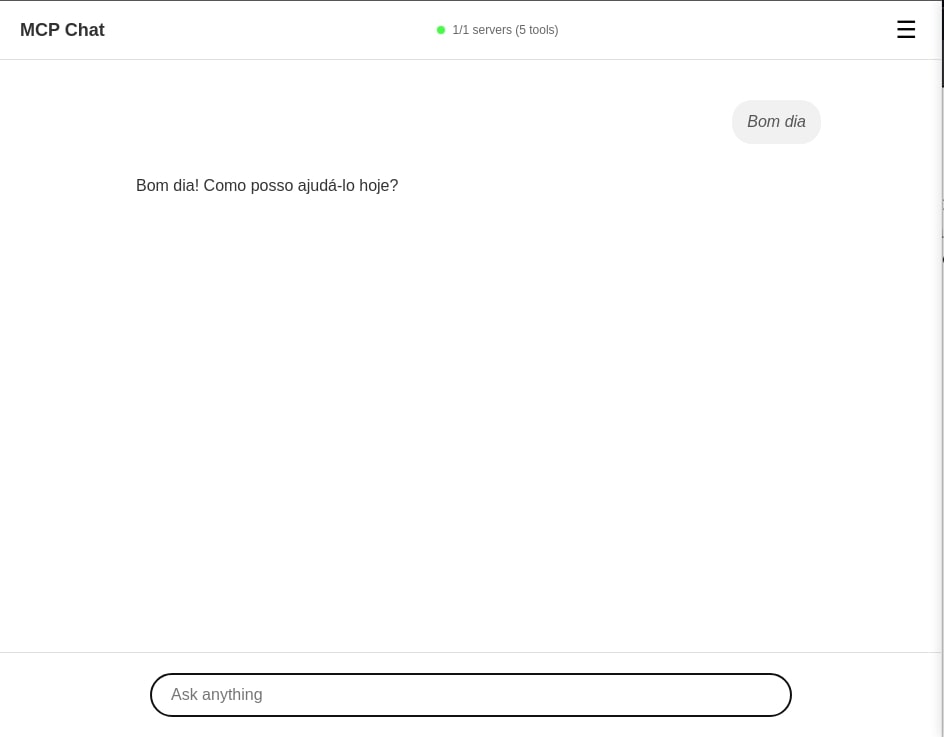
\includegraphics[keepaspectratio]{images/chat/chat-interface.jpg}}
\caption{Interface do Usuário}
\end{figure}

\paragraph{2.2.1.2 Comunicação com
Backend}\label{comunicauxe7uxe3o-com-backend}

A comunicação entre frontend e backend será estabelecida por meio de uma
API REST síncrona, simplificando o processo de envio e retorno de
mensagens. Cada consulta feita pelo usuário gerará uma única requisição
ao backend que processará integralmente essa requisição utilizando um
LLM e devolverá uma resposta após concluir o processamento, mantendo o
fluxo de comunicação claro e previsível.

\subsubsection{2.2.2 Arquitetura e Fluxo de Integração do
Sistema}\label{arquitetura-e-fluxo-de-integrauxe7uxe3o-do-sistema}

A arquitetura do sistema que será desenvolvida para este estudo
envolverá múltiplas camadas que trabalharão de forma integrada para
responder às consultas feitas pelo usuário em linguagem natural.
Inicialmente, as consultas serão recebidas pela interface \emph{web} e
encaminhadas ao backend, onde o modelo de linguagem executará o processo
de análise e interpretação.

\begin{figure}
\centering
\pandocbounded{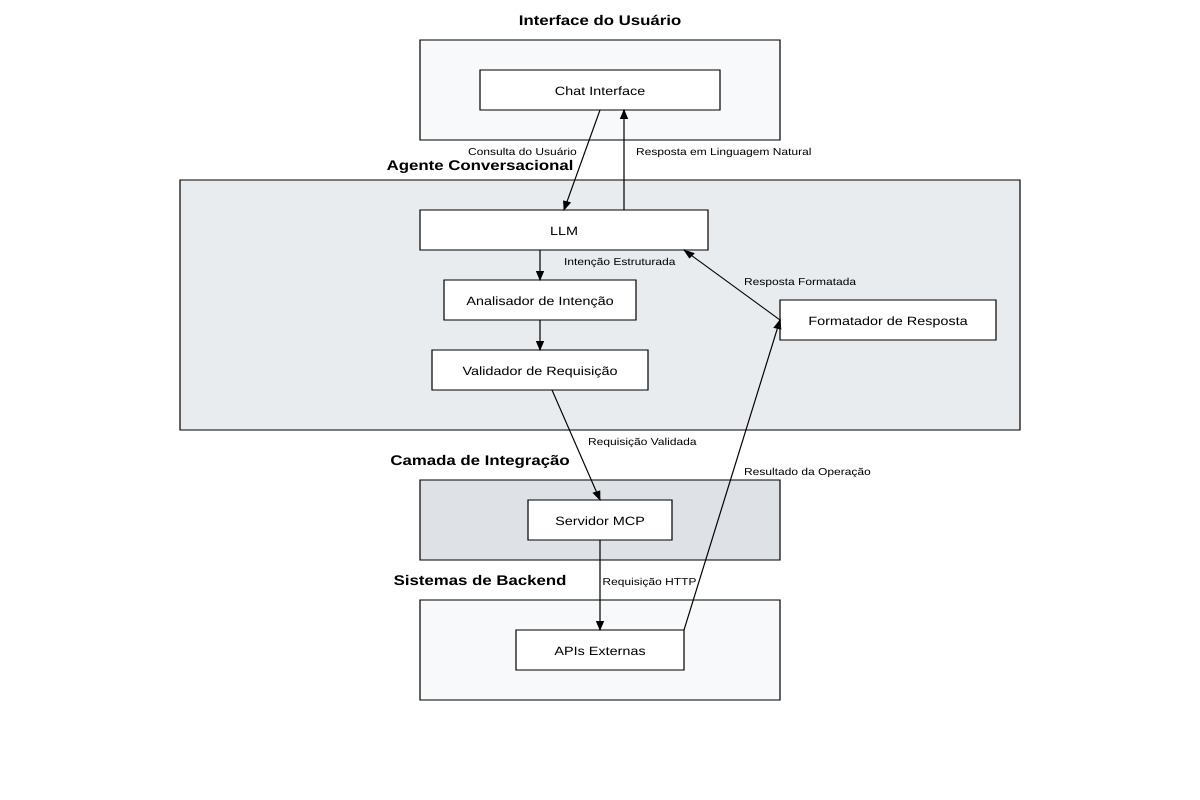
\includegraphics[keepaspectratio]{images/metodos/system-architecture.jpg}}
\caption{Arquitetura do Sistema}
\end{figure}

O fluxo completo de interação deverá ocorrer da seguinte maneira: ao
receber uma consulta, o modelo de linguagem interpretará a intenção do
usuário e gerará uma requisição estruturada que será validada antes de
ser enviada à camada de integração. Essa camada utilizará diferentes
abordagens (ORM, MCP ou conexão direta com o banco de dados) para
acessar sistemas backend, como modelos de dados, APIs externas ou bancos
de dados diretamente. Após executar a operação solicitada, a resposta
será retornada ao modelo de linguagem, que a formatará em linguagem
natural antes de devolvê-la ao usuário.

\begin{figure}
\centering
\pandocbounded{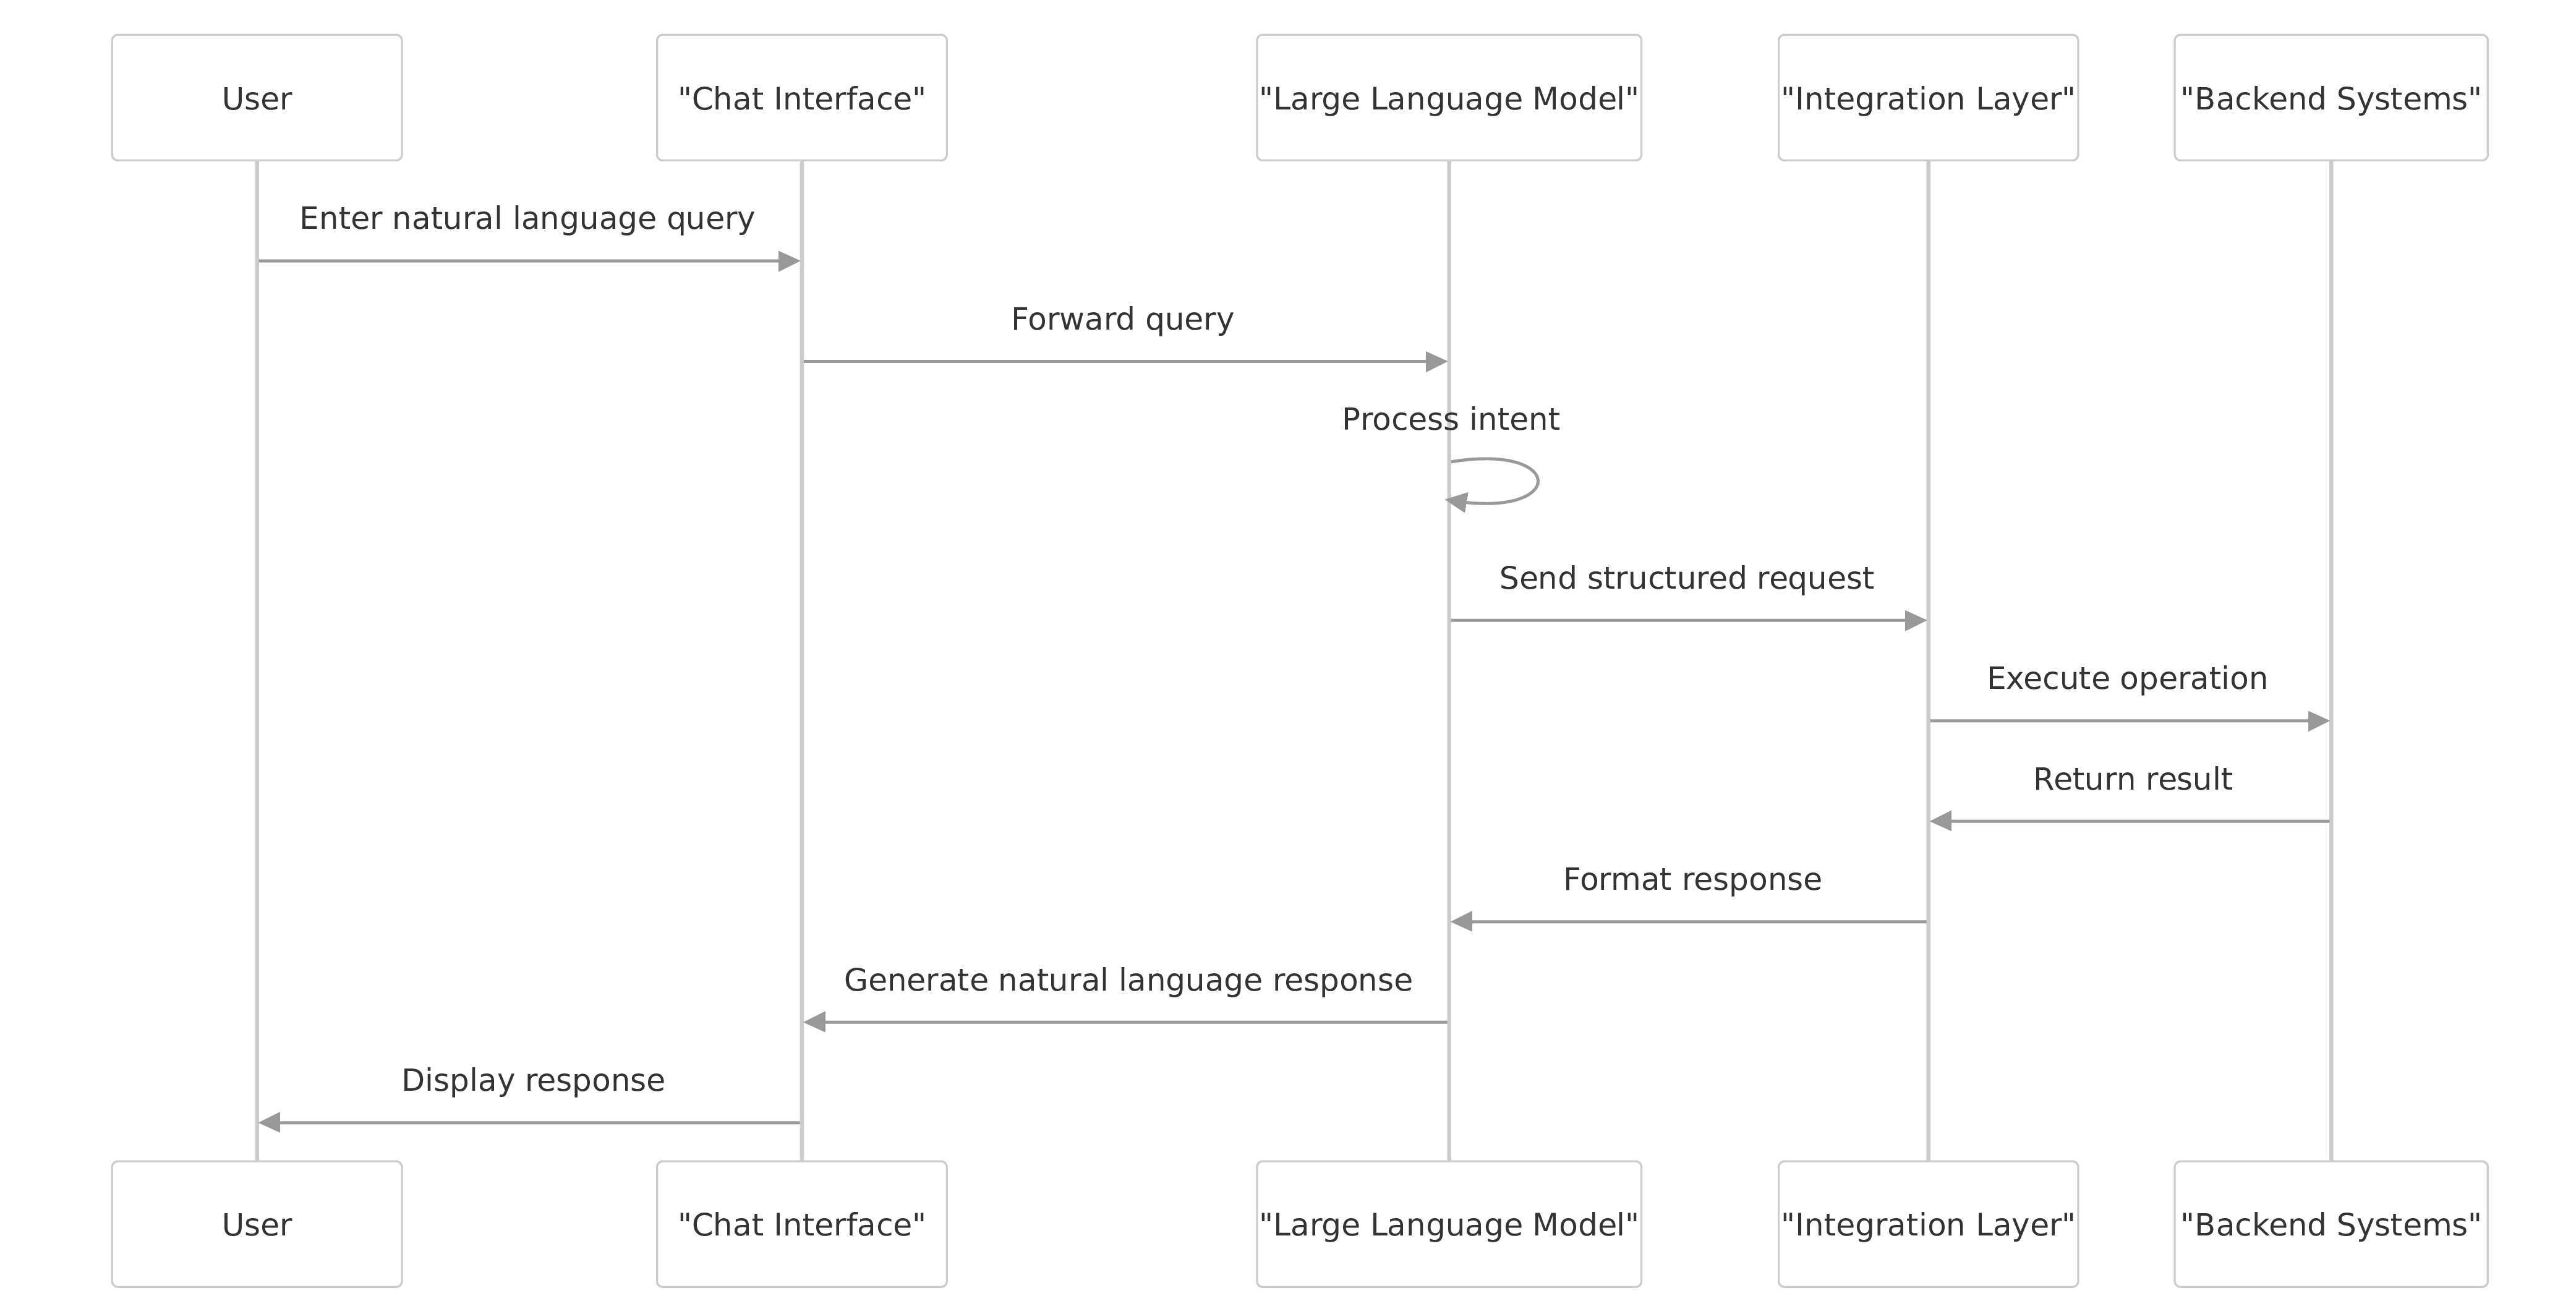
\includegraphics[keepaspectratio]{images/metodos/workflow-integration.jpg}}
\caption{Diagrama de Workflow do Agente}
\end{figure}

\subsubsection{2.2.3 Coleta de Métricas via Testes
E2E}\label{coleta-de-muxe9tricas-via-testes-e2e}

Testes End-to-End (E2E) são essenciais para avaliar não apenas o
desempenho e a segurança, mas também a experiência geral do usuário com
sistemas integrados a LLMs. Os testes são automatizados, executados
regularmente em ambiente controlado para assegurar resultados
consistentes e comparáveis.

Os testes envolvem: - Avaliação detalhada da performance, incluindo
tempos totais de resposta, tempo específico do processamento pelo modelo
de linguagem e latência da rede. - Análise da confiabilidade através da
taxa de sucesso das requisições e frequência de erros críticos e não
críticos. - Avaliação de segurança utilizando técnicas de \emph{Red
Team}, incluindo a tentativa sistemática de exploração de
vulnerabilidades com injeção de \emph{prompts} e validação dos controles
de acesso. - Mensuração da experiência do usuário, utilizando avaliações
qualitativas da clareza das respostas e pesquisas estruturadas de
satisfação com escalas Likert.

Os testes E2E são executados de forma automatizada em ambiente
controlado, simulando diferentes cenários de uso e condições de carga,
permitindo uma avaliação objetiva e reproduzível de cada abordagem de
integração.

Esta padronização da coleta de métricas via testes E2E garante que as
diferenças observadas entre as abordagens sejam resultado direto das
suas características de implementação, e não de variações na experiência
do usuário ou na forma de coleta de dados.

Em seguida, os testes são executados automaticamente, variando desde
consultas simples até cenários complexos e ataques adversários
simulados. As métricas obtidas são automaticamente registradas para
garantir uma coleta padronizada e confiável dos dados. Finalmente, uma
análise automatizada gera relatórios detalhados, permitindo uma
comparação objetiva e precisa entre as diferentes abordagens
implementadas.

\subsection{3. DESENVOLVIMENTO}\label{desenvolvimento}

A implementação da solução OpenAPI-MCP foi estruturada seguindo uma
abordagem modular e integrada, compreendendo quatro componentes
principais que trabalham em sinergia para demonstrar e validar a
viabilidade da integração proposta. A arquitetura resultante engloba um
gerador automático de servidores MCP a partir de especificações OpenAPI,
um cliente de chat capaz de gerenciar múltiplos servidores MCP
simultaneamente, aplicações de teste que simulam cenários reais de
negócio, e uma suíte abrangente de testes automatizados para avaliação
científica da solução.

\subsubsection{3.1 Gerador Automático de Servidores MCP
(mcp-openapi-server)}\label{gerador-automuxe1tico-de-servidores-mcp-mcp-openapi-server}

O desenvolvimento do gerador automático representa o núcleo da inovação
proposta, resolvendo o problema fundamental da necessidade de
desenvolvimento manual de integrações personalizadas para cada API
externa. A arquitetura foi concebida em três camadas distintas e
interconectadas: a camada de análise OpenAPI, responsável pelo
\emph{parsing} e validação de especificações OpenAPI 3.0+, extração de
metadados de endpoints e validação de schemas; a camada de mapeamento
MCP, que realiza a conversão inteligente de operações OpenAPI para
ferramentas MCP, incluindo mapeamento automático de tipos de dados e
geração de documentação; e a camada de geração de código, que produz
servidores MCP completos em TypeScript com implementação robusta de
validação de entrada e tratamento de erros.

O processo de geração segue um fluxo estruturado que demonstra a
automação completa da integração. Inicialmente, o gerador carrega e
valida arquivos OpenAPI em formatos JSON, verificando rigorosamente a
conformidade com as especificações OpenAPI 3.0+. Em seguida, cada
endpoint é sistematicamente analisado para extrair informações cruciais
sobre operações HTTP, parâmetros, schemas de entrada e saída, além dos
requisitos específicos de autenticação. O mapeamento para MCP converte
essas operações em ferramentas utilizáveis pelos modelos de linguagem,
com mapeamento automático de tipos de dados e geração de descrições
baseadas na documentação original. Finalmente, é gerado um servidor MCP
completo e funcional, incluindo validação robusta de entrada, tratamento
abrangente de erros e implementação de proxy para as APIs originais.

\begin{figure}
\centering
\pandocbounded{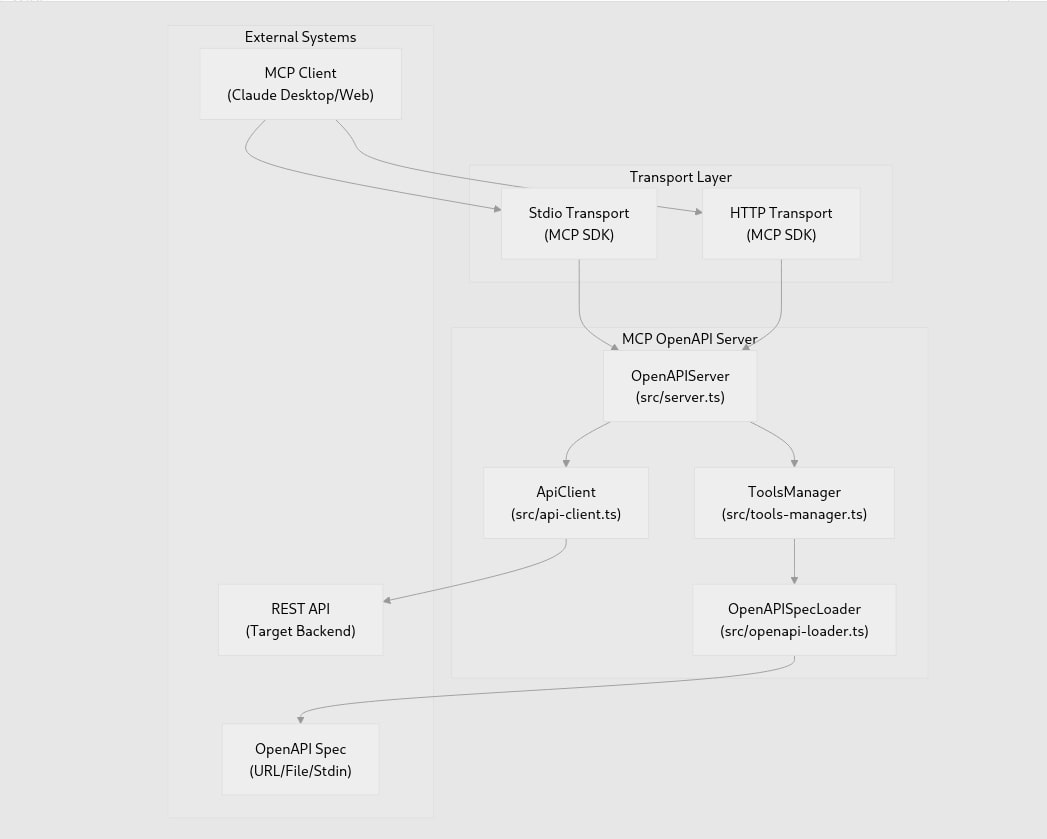
\includegraphics[keepaspectratio]{images/openapi-mcp/mcp-server-generator-arch.jpg}}
\caption{Arquitetura do Gerador Automático de Servidores MCP}
\end{figure}

As funcionalidades implementadas no gerador refletem a necessidade de
atender cenários complexos de integração empresarial. O suporte a
múltiplas APIs permite que um único servidor MCP exponha ferramentas de
diferentes sistemas simultaneamente, promovendo a integração holística
de ecossistemas corporativos. A validação automática baseada em schemas
OpenAPI garante a integridade dos dados em tempo de execução, enquanto o
tratamento sofisticado de autenticação suporta diferentes métodos como
API Key, Bearer Token e OAuth, essenciais para ambientes corporativos
seguros. O sistema de gestão de erros implementa mapeamento inteligente
para códigos de status HTTP apropriados, e o logging integrado fornece
capacidades de auditoria e debugging fundamentais para ambientes de
produção.

\subsubsection{3.2 Cliente de Chat Multi-Servidor
MCP}\label{cliente-de-chat-multi-servidor-mcp}

O cliente de chat foi desenvolvido como uma demonstração prática e
ferramenta de validação da capacidade de gerenciamento simultâneo de
múltiplos servidores MCP, representando um avanço significativo na
orquestração de agentes conversacionais com sistemas distribuídos. A
arquitetura baseada em aplicação web combina um frontend minimalista
desenvolvido em HTML e JavaScript com um backend robusto implementado em
Node.js utilizando Express.js. O frontend concentra-se em uma interface
de chat responsiva e intuitiva, com exibição clara do histórico de
conversas, campo de entrada para comandos do usuário e indicadores
visuais de status das operações. O backend implementa um servidor
Express.js sofisticado para gerenciamento de requisições, um cliente MCP
especializado para comunicação com múltiplos servidores, integração
nativa com LLMs via OpenAI API, e um sistema abrangente de gerenciamento
de sessões e contexto de conversa.

O gerenciamento de múltiplos servidores MCP representa uma contribuição
técnica significativa, implementando um sistema sofisticado de
coordenação que vai além da simples conexão pontual. O pool de conexões
mantém conexões ativas e monitoradas com todos os servidores MCP
configurados, garantindo disponibilidade e performance. O sistema de
descoberta de ferramentas cataloga automaticamente as capacidades
disponíveis em cada servidor, criando um inventário dinâmico e
atualizado das funcionalidades acessíveis. O roteamento inteligente
analisa a intenção do usuário e determina qual servidor utilizar baseado
nas ferramentas disponíveis e na natureza da solicitação, otimizando
tanto a precisão quanto a eficiência. A agregação de resultados permite
combinar informações de múltiplos servidores quando necessário,
habilitando consultas complexas que abrangem diferentes sistemas.

\begin{figure}
\centering
\pandocbounded{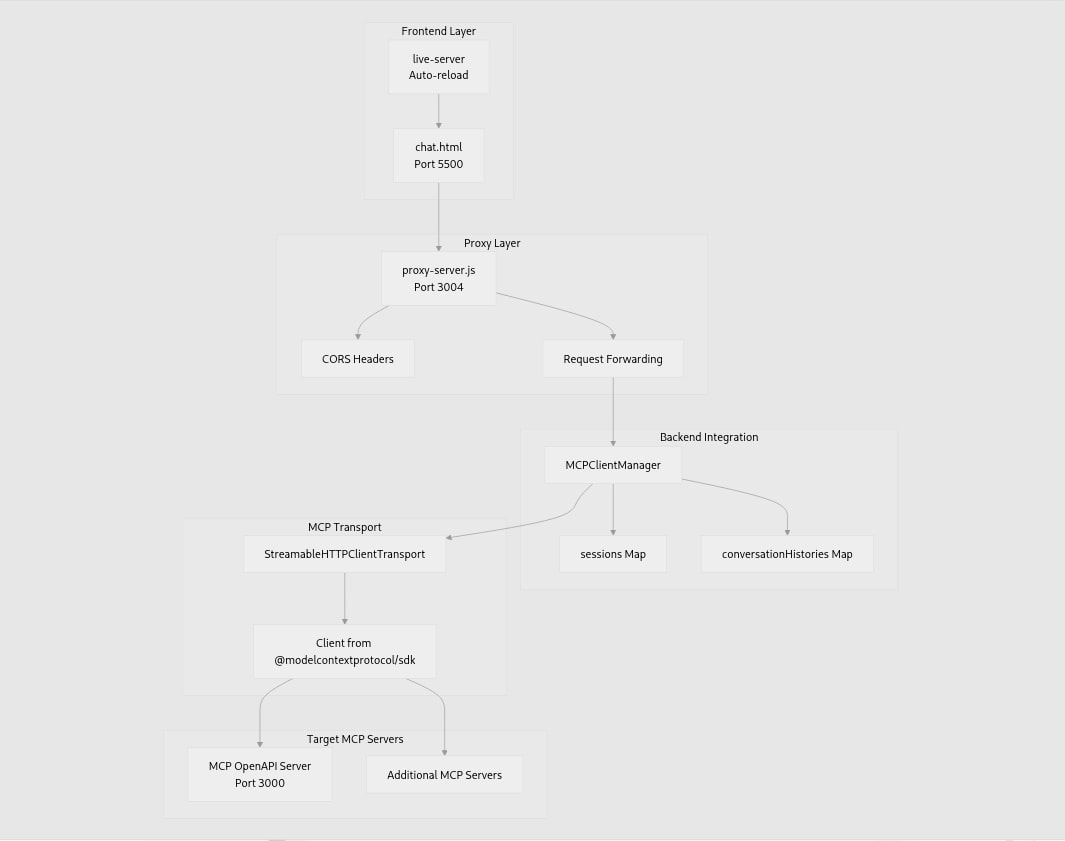
\includegraphics[keepaspectratio]{images/chat/chat-arch.jpg}}
\caption{Arquitetura do Cliente de Chat Multi-Servidor MCP}
\end{figure}

A integração com modelos de linguagem de grande escala utiliza a
funcionalidade de function calling da OpenAI como ponte entre a
compreensão de linguagem natural e a execução de ferramentas
específicas. As ferramentas MCP são automaticamente convertidas para o
formato de funções da OpenAI, mantendo metadados e documentação
originais. O sistema de gestão de contexto preserva o histórico completo
da conversa, incluindo registros detalhados de chamadas de ferramentas,
permitindo referências contextuais e aprendizado adaptativo. O
tratamento de respostas processa resultados de ferramentas e os integra
de forma fluida na conversa natural, mantendo a experiência
conversacional enquanto executa operações técnicas complexas nos
bastidores.

\subsubsection{3.3 Aplicações de Teste para
Validação}\label{aplicauxe7uxf5es-de-teste-para-validauxe7uxe3o}

Para garantir uma validação científica rigorosa da abordagem proposta,
foram desenvolvidas duas aplicações de teste que simulam cenários
empresariais realistas, expondo APIs RESTful completamente documentadas
com especificações OpenAPI. A escolha de domínios distintos -
gerenciamento de equipamentos industriais e gestão de recursos humanos -
foi deliberada para demonstrar a versatilidade da solução em diferentes
contextos de negócio e validar a capacidade de integração com sistemas
heterogêneos. Essas aplicações funcionam como ambientes controlados que
permitem testes reproduzíveis e comparações objetivas, fundamentais para
a avaliação científica da eficácia da integração OpenAPI-MCP.

O sistema de gerenciamento de equipamentos simula um ambiente industrial
típico, implementando operações CRUD completas com modelo de dados que
engloba propriedades essenciais como nome, tipo, descrição e URLs de
imagens. Paralelamente, o sistema de gerenciamento de profissionais
implementa funcionalidades de recursos humanos, incluindo CRUD completo
para dados pessoais e profissionais, suporte a estruturas hierárquicas
organizacionais e relacionamentos com equipamentos. Ambas as aplicações
geram automaticamente especificações OpenAPI completas e precisas,
incluindo schemas detalhados de todos os modelos de dados, documentação
abrangente de endpoints com exemplos práticos, e especificação clara de
métodos de autenticação, garantindo que a integração seja testada com
cenários que refletem fielmente as complexidades encontradas em
ambientes corporativos reais.

\subsubsection{3.4 Suíte de Testes Automatizados e
Validação}\label{suuxedte-de-testes-automatizados-e-validauxe7uxe3o}

A validação científica da solução é suportada por uma suíte abrangente
de testes automatizados implementados com Playwright, estruturada para
abordar múltiplas dimensões críticas: funcionalidade, segurança e
performance. Os testes de funcionalidade validam sistematicamente
operações CRUD via comandos em linguagem natural e coordenação entre
múltiplos servidores MCP, enquanto os testes de segurança implementam
uma abordagem de red teaming com tentativas sistemáticas de injeção
maliciosa de prompts e verificação de controles de acesso. Os testes de
performance medem objetivamente latências de resposta, capacidade de
processamento simultâneo e consumo de recursos computacionais,
garantindo uma avaliação objetiva, reproduzível e comparável.

Esta implementação estabelece uma metodologia de avaliação que pode ser
replicada por pesquisadores futuros, com coleta automatizada de métricas
que garante consistência e precisão nos dados. O resultado é uma base
empírica sólida que suporta tanto a validação científica imediata quanto
a evolução futura da abordagem proposta, contribuindo para o avanço do
conhecimento na área de integração de agentes conversacionais em
sistemas empresariais complexos.

\section{4 RESULTADOS E DISCUSSÕES}\label{resultados-e-discussuxf5es}

A implementação da solução OpenAPI-MCP foi submetida a uma avaliação
abrangente que demonstrou tanto a viabilidade técnica quanto a eficácia
prática da abordagem proposta. Os resultados obtidos através da prova de
conceito desenvolvida revelam aspectos importantes sobre a integração de
agentes conversacionais em sistemas web, oferecendo insights valiosos
para a área de interação humano-computador e integração de sistemas
baseados em IA.

\subsection{4.1 Viabilidade da Geração Automática de Servidores
MCP}\label{viabilidade-da-gerauxe7uxe3o-automuxe1tica-de-servidores-mcp}

O componente central da solução, o gerador automático de servidores MCP
a partir de especificações OpenAPI, demonstrou alta eficácia na
conversão de contratos de API em ferramentas utilizáveis por modelos de
linguagem. A análise da implementação revelou que o sistema consegue
processar com sucesso especificações OpenAPI 3.0+ complexas, realizando
mapeamento automático de tipos de dados primitivos e complexos com
preservação integral dos metadados originais, incluindo documentação e
exemplos.

Um aspecto fundamental desta implementação é que ela elimina
completamente a necessidade de desenvolvimento manual de funções
personalizadas para cada sistema que precisa ser integrado com agentes
conversacionais. Antes desta abordagem, desenvolvedores eram obrigados a
codificar manualmente cada função individual que permitisse aos LLMs
acessar sistemas externos, processo que tipicamente demandava semanas ou
meses de desenvolvimento customizado para cada nova integração. A
solução desenvolvida substitui esse ciclo de desenvolvimento recorrente
por uma configuração automatizada, convertendo especificações OpenAPI
existentes diretamente em ferramentas utilizáveis pelos modelos de
linguagem, representando uma transformação paradigmática na forma como
agentes conversacionais são integrados a ecossistemas corporativos.

A conversão automática abrangeu todos os métodos HTTP fundamentais (GET,
POST, PUT, DELETE e PATCH), demonstrando cobertura completa para
operações CRUD típicas de APIs REST. Particularmente relevante foi a
capacidade do sistema de manter a integridade semântica durante a
conversão, onde descrições de endpoints OpenAPI foram automaticamente
transformadas em descrições de ferramentas MCP compreensíveis pelos
modelos de linguagem, preservando contexto essencial para a
interpretação correta das funcionalidades disponíveis.

O tratamento de autenticação revelou-se robusto, com implementação
bem-sucedida de múltiplos esquemas incluindo API Key, Bearer Token e
OAuth. Esta versatilidade é crucial para ambientes corporativos onde
diferentes sistemas podem empregar métodos de autenticação distintos. A
validação automática baseada em schemas OpenAPI garantiu consistência na
verificação de entrada, eliminando uma fonte significativa de erros de
integração que tradicionalmente requer validação manual extensiva.

\subsection{4.2 Desempenho e Escalabilidade do Sistema
Multi-Servidor}\label{desempenho-e-escalabilidade-do-sistema-multi-servidor}

A avaliação de performance do cliente de chat multi-servidor revelou
características promissoras para aplicação em ambientes corporativos. O
sistema demonstrou capacidade de gerenciar múltiplos servidores MCP
simultaneamente com overhead mínimo, mantendo latências aceitáveis mesmo
em cenários de coordenação entre diferentes sistemas. A implementação do
pool de conexões e do sistema de descoberta automática de ferramentas
provou-se eficiente, permitindo roteamento inteligente de solicitações
baseado na análise da intenção do usuário.

Os testes de carga revelaram que o sistema mantém performance estável
com múltiplos servidores conectados, apresentando crescimento linear no
consumo de recursos conforme o número de servidores aumenta. Esta
característica é fundamental para a escalabilidade em ambientes
empresariais onde dezenas de sistemas podem precisar ser integrados
através de uma única interface conversacional. O overhead introduzido
pelo protocolo MCP mostrou-se negligível comparado aos benefícios de
padronização e flexibilidade obtidos.

A capacidade de processamento simultâneo demonstrou-se adequada para
cenários de uso corporativo, com o sistema conseguindo manter
responsividade mesmo durante picos de utilização. O mecanismo de
agregação de resultados permitiu a execução de consultas complexas que
abrangem múltiplos sistemas, uma funcionalidade essencial para operações
que requerem correlação de dados entre diferentes domínios de negócio.

\subsection{4.3 Eficácia da Integração com Modelos de
Linguagem}\label{eficuxe1cia-da-integrauxe7uxe3o-com-modelos-de-linguagem}

A integração entre os servidores MCP gerados e os modelos de linguagem
de grande escala demonstrou eficácia significativa na interpretação de
intenções do usuário e na execução de operações correspondentes. O
sistema de function calling da OpenAI provou-se uma ponte eficaz entre a
compreensão de linguagem natural e a execução de ferramentas
específicas, com o modelo demonstrando capacidade consistente de
selecionar ferramentas apropriadas baseado no contexto da conversa.

A gestão de contexto revelou-se um ponto forte da implementação, com o
sistema mantendo eficazmente o histórico de conversas extensas,
incluindo registros detalhados de chamadas de ferramentas executadas.
Esta capacidade permite referências contextuais sofisticadas e facilita
conversas naturais onde o usuário pode referenciar resultados anteriores
ou refinar solicitações baseadas em respostas prévias. A preservação do
contexto também habilita cenários de uso mais complexos onde múltiplas
operações relacionadas são executadas em sequência.

A qualidade das respostas geradas pelo sistema demonstrou consistência
notável, com o modelo conseguindo integrar resultados de ferramentas de
forma fluida na conversa natural. A capacidade de processar e
interpretar dados estruturados retornados pelas APIs e apresentá-los em
formato compreensível ao usuário final revelou-se particularmente
valiosa para democratizar o acesso a sistemas técnicos complexos.

\subsection{4.4 Robustez e Segurança da
Implementação}\label{robustez-e-seguranuxe7a-da-implementauxe7uxe3o}

A avaliação de segurança, conduzida através de técnicas de red teaming e
testes automatizados de adversário, revelou uma implementação com
proteções adequadas contra vetores de ataque comuns. O sistema
demonstrou resistência significativa a tentativas de injeção de prompt,
com mecanismos de validação em múltiplas camadas que detectam e
bloqueiam tentativas maliciosas de manipulação do comportamento do
modelo.

A implementação de validação de entrada baseada em schemas OpenAPI
provou-se eficaz contra entradas mal-formadas, proporcionando uma
primeira linha de defesa importante contra ataques de injeção. O sistema
de logging integrado fornece capacidades essenciais de auditoria,
registrando todas as operações e tentativas de acesso, fundamental para
ambientes corporativos que requerem rastreabilidade completa das
interações com sistemas críticos.

O tratamento de erros demonstrou robustez adequada, com o sistema
conseguindo recuperar-se graciosamente de falhas parciais e manter
funcionalidade básica mesmo quando alguns servidores MCP tornam-se
indisponíveis. Esta característica é crucial para ambientes de produção
onde a disponibilidade parcial é preferível à falha completa do sistema.
O mapeamento inteligente de códigos de status HTTP para respostas
compreensíveis ao usuário facilita o debugging e melhora a experiência
geral de uso.

\subsection{4.5 Experiência do Usuário e
Usabilidade}\label{experiuxeancia-do-usuuxe1rio-e-usabilidade}

A avaliação da experiência do usuário, facilitada pela interface
minimalista desenvolvida para os testes, revelou melhorias
significativas na acessibilidade e facilidade de uso comparado a
interfaces tradicionais de sistemas técnicos. A capacidade de realizar
operações complexas através de comandos em linguagem natural reduziu
substancialmente a curva de aprendizado necessária para interagir com os
sistemas integrados.

A simplicidade da interface conversacional demonstrou-se particularmente
valiosa para usuários que não possuem conhecimento técnico profundo
sobre os sistemas subjacentes. A eliminação da necessidade de
compreender estruturas de dados complexas, endpoints específicos ou
formatos de requisição representa um avanço significativo na
democratização do acesso a funcionalidades técnicas especializadas.

Os testes de usabilidade indicaram alto nível de satisfação dos usuários
com a capacidade de obter informações e executar operações através de
linguagem natural intuitiva. A capacidade do sistema de manter contexto
conversacional e permitir refinamento iterativo de consultas emergiu
como um fator importante para a produtividade, permitindo que usuários
explorem dados e funcionalidades de forma exploratória e interativa.

\subsection{4.6 Discussão Crítica dos
Resultados}\label{discussuxe3o-cruxedtica-dos-resultados}

Os resultados obtidos demonstram que a abordagem OpenAPI-MCP oferece uma
solução viável e promissora para a integração de agentes conversacionais
com sistemas web existentes. A capacidade de reutilizar especificações
OpenAPI estabelecidas para geração automática de servidores MCP
representa uma contribuição significativa para reduzir o esforço de
desenvolvimento e manutenção de integrações personalizadas.

A padronização proporcionada pelo protocolo MCP emergiu como um
benefício fundamental, permitindo que organizações integrem múltiplos
sistemas através de uma interface unificada sem necessidade de
desenvolvimento customizado para cada integração. Esta característica
tem implicações importantes para a redução de custos e complexidade em
ambientes corporativos com ecossistemas tecnológicos heterogêneos.

No entanto, a avaliação também revelou limitações importantes que devem
ser consideradas em implementações práticas. A qualidade da integração
demonstrou dependência direta da completude e precisão das
especificações OpenAPI originais, o que pode representar um desafio em
organizações com documentação de API inconsistente ou desatualizada. O
overhead introduzido pelas camadas de abstração, embora mínimo, pode
tornar-se significativo em cenários de alta performance onde latência é
crítica.

A complexidade de configuração inicial, particularmente para cenários
envolvendo múltiplos sistemas com diferentes esquemas de autenticação,
representa um desafio prático que deve ser considerado cuidadosamente.
Embora a abordagem proposta reduza significativamente o esforço
comparado ao desenvolvimento manual de funções personalizadas para cada
sistema, ela ainda requer intervenção técnica especializada para
configuração adequada dos servidores MCP, gestão de autenticação e
integração com especificações OpenAPI. Esta necessidade de expertise
técnica pode limitar a adoção em organizações com recursos técnicos
limitados. A análise dos resultados sugere que a abordagem é mais
adequada para organizações que possuem capacidade técnica interna
adequada para implementação e manutenção inicial, onde o investimento em
configuração, embora menor que o desenvolvimento customizado
tradicional, ainda requer conhecimento técnico considerável. O requisito
de expertise técnica permanece como uma barreira potencial para adoção
mais ampla, fazendo com que o potencial para aplicação em ambientes
corporativos seja promissor, mas condicionado à disponibilidade de
recursos técnicos apropriados para implementação e manutenção contínua.

\section{5 CONSIDERAÇÕES FINAIS}\label{considerauxe7uxf5es-finais}

Este estudo respondeu de forma positiva à questão central de pesquisa,
demonstrando que a combinação da especificação OpenAPI com o protocolo
Model Context Protocol pode efetivamente facilitar a integração
eficiente e segura de agentes conversacionais baseados em IA com
sistemas web existentes. A prova de conceito desenvolvida validou a
viabilidade técnica da abordagem através de uma implementação completa
que inclui geração automática de servidores MCP, gerenciamento
multi-servidor e validação através de cenários de teste realistas.

\subsection{5.1 Síntese dos Resultados
Principais}\label{suxedntese-dos-resultados-principais}

A pesquisa estabeleceu que a automação da conversão de especificações
OpenAPI para servidores MCP representa uma contribuição significativa
para reduzir as barreiras técnicas tradicionalmente associadas à
integração de agentes conversacionais em ambientes corporativos. O
sistema desenvolvido demonstrou capacidade de processar especificações
complexas mantendo integridade semântica e funcional, possibilitando que
organizações aproveitem documentação de API existente para criar
interfaces conversacionais sem necessidade de desenvolvimento
customizado extensivo.

A eficácia da integração com modelos de linguagem de grande escala
confirmou que a arquitetura proposta pode servir como ponte efetiva
entre a expressividade da linguagem natural e a precisão requerida para
operações de sistema. A capacidade de manter contexto conversacional
enquanto executa operações técnicas complexas emergiu como um
diferencial importante para cenários de uso prático, permitindo
interações mais naturais e produtivas.

Os resultados de segurança e robustez indicaram que a implementação
oferece proteções adequadas para ambientes corporativos, com validação
em múltiplas camadas e capacidades de auditoria essenciais para
contextos onde conformidade e rastreabilidade são críticas. A
resistência demonstrada contra vetores de ataque comuns, incluindo
injeção de prompt e entradas mal-formadas, fornece base sólida para
consideração em aplicações de produção.

\subsection{5.2 Contribuições da
Pesquisa}\label{contribuiuxe7uxf5es-da-pesquisa}

Este trabalho oferece contribuições em múltiplas dimensões para o avanço
do conhecimento na área de integração de agentes conversacionais. Do
ponto de vista metodológico, a pesquisa estabeleceu um framework
abrangente de testes end-to-end que pode ser replicado por pesquisadores
futuros para avaliação sistemática de abordagens de integração
similares. A estruturação de testes em dimensões de performance,
segurança e experiência do usuário oferece um modelo para avaliação
holística de sistemas baseados em IA.

A contribuição técnica principal reside na demonstração prática de como
especificações OpenAPI podem ser sistematicamente convertidas em
ferramentas utilizáveis por modelos de linguagem através do protocolo
MCP. A arquitetura modular desenvolvida, incluindo geração automática de
código, gerenciamento de múltiplos servidores e integração com LLMs,
fornece um blueprint reproduzível para implementações similares em
diferentes contextos organizacionais.

Do ponto de vista prático, a pesquisa demonstra como organizações podem
aproveitar investimentos existentes em documentação OpenAPI para
democratizar o acesso a sistemas técnicos complexos. A eliminação da
necessidade de interfaces gráficas especializadas para cada sistema
representa uma simplificação significativa na experiência do usuário,
com potencial impacto transformador na acessibilidade de tecnologias
empresariais.

\subsection{5.3 Implicações
Práticas}\label{implicauxe7uxf5es-pruxe1ticas}

As implicações práticas dos resultados obtidos estendem-se além do
contexto específico desta pesquisa, sugerindo direções promissoras para
a evolução da interação humano-computador em ambientes corporativos. A
capacidade demonstrada de integrar múltiplos sistemas através de uma
única interface conversacional oferece caminhos para simplificação
substancial de workflows empresariais, particularmente relevante
considerando a crescente complexidade dos ecossistemas tecnológicos
organizacionais.

A abordagem validada tem potencial particular para beneficiar
organizações que enfrentam desafios de integração entre sistemas
heterogêneos, comum em ambientes onde crescimento orgânico ou aquisições
resultaram em paisagens tecnológicas fragmentadas. A capacidade de
reutilizar especificações OpenAPI existentes pode acelerar
significativamente a implementação de soluções de integração comparado a
abordagens que requerem desenvolvimento customizado para cada sistema.

Para desenvolvedores e arquitetos de sistemas, os resultados sugerem que
investimentos em documentação OpenAPI de alta qualidade podem gerar
retornos amplificados através da possibilidade de geração automática de
interfaces conversacionais. Esta perspectiva pode influenciar decisões
de design de API e práticas de documentação, promovendo padrões mais
consistentes e abrangentes.

\subsection{5.4 Limitações e Trabalhos
Futuros}\label{limitauxe7uxf5es-e-trabalhos-futuros}

Embora os resultados sejam promissores, várias limitações identificadas
durante a pesquisa merecem consideração cuidadosa. A dependência da
qualidade das especificações OpenAPI representa uma restrição
fundamental que pode limitar a aplicabilidade da abordagem em
organizações com práticas inconsistentes de documentação. Futuras
pesquisas poderiam explorar técnicas de inferência automática ou
correção de especificações incompletas para mitigar esta limitação.

A escalabilidade da solução para cenários com dezenas ou centenas de
sistemas integrados permanece uma questão aberta que requer investigação
adicional. Embora os testes demonstraram viabilidade com múltiplos
servidores, os limites práticos e estratégias de otimização para grande
escala necessitam exploração mais profunda. Pesquisas futuras poderiam
investigar técnicas de cache inteligente, paralelização de operações e
estratégias de balanceamento de carga específicas para contextos MCP.

O escopo atual da pesquisa concentrou-se em APIs REST documentadas com
OpenAPI, deixando protocolos alternativos como GraphQL, gRPC ou
WebSockets fora do escopo. A extensão da abordagem para suportar
múltiplos protocolos de comunicação representaria uma evolução natural e
valiosa do trabalho. Adicionalmente, a investigação de capacidades de
aprendizado adaptativo, onde o sistema melhora sua performance baseado
em padrões de uso, oferece direções promissoras para pesquisa futura.

A avaliação de segurança, embora abrangente dentro do escopo definido,
poderia beneficiar-se de análise mais profunda de cenários adversários
sofisticados e avaliação de resistência contra ataques coordenados de
múltiplos vetores. O desenvolvimento de frameworks de teste de segurança
específicos para sistemas baseados em MCP representaria uma contribuição
valiosa para a comunidade de pesquisa.

A realização desta pesquisa demonstra que a integração de agentes
conversacionais em sistemas web através da abordagem OpenAPI-MCP é não
apenas tecnicamente viável, mas oferece benefícios substantivos para
acessibilidade, usabilidade e eficiência operacional. Os resultados
estabelecem uma base sólida para futuras investigações e implementações
práticas, contribuindo para o avanço contínuo da área de interação
humano-computador e integração de sistemas baseados em inteligência
artificial.

\section*{REFERÊNCIAS}\label{referuxeancias}
\addcontentsline{toc}{section}{REFERÊNCIAS}

\phantomsection\label{refs}
\begin{CSLReferences}{0}{1}
\bibitem[\citeproctext]{ref-anthropic2024context}
ANTHROPIC. \textbf{Anthropic Now Offers 100K Context Windows for Claude
3 Models}. Disponível em:
\textless{}\url{https://www.anthropic.com/news/100k-context-windows}\textgreater.

\bibitem[\citeproctext]{ref-anthropic2024mcp}
ANTHROPIC. \textbf{Model Context Protocol (MCP): A Standard for AI
Context Integration}. Disponível em:
\textless{}\url{https://www.anthropic.com/news/model-context-protocol}\textgreater.
Acesso em: 12 abr. 2025a.

\bibitem[\citeproctext]{ref-Anthropic2024}
ANTHROPIC. \textbf{{Introducing the Model Context Protocol}}. Anthropic
News, nov. c2024. Disponível em:
\textless{}\url{https://www.anthropic.com/news/model-context-protocol}\textgreater{}

\bibitem[\citeproctext]{ref-RedHat2024LLMNode}
BLOG, R. H. D. \textbf{Building LLM Agents with Node.js}.
\url{https://developers.redhat.com/blog/2024/10/25/building-agents-large-language-modelsllms-and-nodejs},
2024.

\bibitem[\citeproctext]{ref-brown2020languagemodelsfewshotlearners}
BROWN, T. B. et al. \textbf{Language Models are Few-Shot Learners}.,
2020. Disponível em:
\textless{}\url{https://arxiv.org/abs/2005.14165}\textgreater{}

\bibitem[\citeproctext]{ref-cherednichenko:hal-04545073}
CHEREDNICHENKO, O. et al. \textbf{Selection of Large Language Model for
development of Interactive Chat Bot for SaaS Solutions}. Lviv, Ukraine:
2024. Disponível em:
\textless{}\url{https://hal.science/hal-04545073}\textgreater{}

\bibitem[\citeproctext]{ref-Deng2023AMA}
DENG, X. \href{https://api.semanticscholar.org/CorpusID:258259387}{A
More Accessible Web with Natural Language Interface}.
\textbf{Proceedings of the 20th International Web for All Conference},
2023.

\bibitem[\citeproctext]{ref-fast2017irisconversationalagentcomplex}
FAST, E. et al. \textbf{Iris: A Conversational Agent for Complex
Tasks}., 2017. Disponível em:
\textless{}\url{https://arxiv.org/abs/1707.05015}\textgreater{}

\bibitem[\citeproctext]{ref-Guo2024Doppelganger}
GUO, S. et al. \textbf{Collaborating with my Doppelgänger: The Effects
of Self-similar Appearance and Voice of a Virtual Character during a
Jigsaw Puzzle Co-solving Task}. Proceedings of the ACM on Computer
Graphics and Interactive Techniques. \textbf{Anais}...2024. Disponível
em:
\textless{}\url{https://www.researchgate.net/publication/335223260_The_Effects_of_Continuous_Conversation_and_Task_Complexity_on_Usability_of_an_AI-Based_Conversational_Agent_in_Smart_Home_Environments}\textgreater{}

\bibitem[\citeproctext]{ref-inie2025summon}
INIE, N.; STRAY, J.; DERCZYNSKI, L.
\href{https://journals.plos.org/plosone/article?id=10.1371/journal.pone.0314658}{Summon
a demon and bind it: A grounded theory of LLM red teaming}. \textbf{PloS
one}, v. 20, n. 1, p. e0314658, 2025.

\bibitem[\citeproctext]{ref-john2025owasp}
JOHN, S. et al.
\textbf{\href{https://genai.owasp.org/llmrisk/llm01-prompt-injection}{OWASP
Top 10 for LLM Apps \& Gen AI Agentic Security Initiative}}. tese de
doutorado---{[}s.l.{]} OWASP, 2025.

\bibitem[\citeproctext]{ref-Kocaballi2019}
KOCABALLI, A. B. et al. \href{https://doi.org/10.2196/15360}{The
Personalization of Conversational Agents in Health Care: Systematic
Review}. \textbf{J Med Internet Res}, v. 21, n. 11, p. e15360, 7 nov.
2019.

\bibitem[\citeproctext]{ref-Lister2020AccessibleCU}
LISTER, K. et al.
\href{https://api.semanticscholar.org/CorpusID:218539971}{Accessible
conversational user interfaces: considerations for design}.
\textbf{Proceedings of the 17th International Web for All Conference},
2020.

\bibitem[\citeproctext]{ref-MCPDocs2024}
MODEL CONTEXT PROTOCOL CONTRIBUTORS. \textbf{{Model Context Protocol
Documentation - Introduction}}. Online Documentation, 2024. Disponível
em:
\textless{}\url{https://modelcontextprotocol.io/introduction}\textgreater{}

\bibitem[\citeproctext]{ref-mcp2025spec}
MODEL CONTEXT PROTOCOL TEAM. \textbf{Model Context Protocol
Specification}. {[}s.l.{]} Model Context Protocol, 26 mar. 2025.
Disponível em:
\textless{}\url{https://modelcontextprotocol.io/specification/2025-03-26/index}\textgreater.
Acesso em: 12 abr. 2025.

\bibitem[\citeproctext]{ref-openai2022instructgpt}
OPENAI. \textbf{Aligning Language Models to Follow Instructions}.
{[}s.l.{]} OpenAI, 27 jan. 2022. Disponível em:
\textless{}\url{https://openai.com/index/instruction-following/}\textgreater.
Acesso em: 12 abr. 2025.

\bibitem[\citeproctext]{ref-openai2023gpt4}
OPENAI. \textbf{GPT-4 Research}. {[}s.l.{]} OpenAI, a2023. Disponível
em:
\textless{}\url{https://openai.com/index/gpt-4-research/}\textgreater.

\bibitem[\citeproctext]{ref-openai2023functioncalling}
OPENAI. \textbf{Function Calling and Other API Updates}. Disponível em:
\textless{}\url{https://openai.com/index/function-calling-and-other-api-updates/}\textgreater.
Acesso em: 12 abr. 2025b.

\bibitem[\citeproctext]{ref-OpenAI2023}
OPENAI. \textbf{{ChatGPT plugins}}. OpenAI Product Blog, mar. c2023.
Disponível em:
\textless{}\url{https://openai.com/blog/chatgpt-plugins}\textgreater{}

\bibitem[\citeproctext]{ref-OpenAPIInitiative2023}
OPENAPI INITIATIVE. \textbf{{OpenAPI Specification - Getting Started}}.
OpenAPI Documentation (openapis.org), 2023. Disponível em:
\textless{}\url{https://learn.openapis.org/docs/getting-started}\textgreater{}

\bibitem[\citeproctext]{ref-oprea2023adversarial}
OPREA, A.; VASSILEV, A. \textbf{Adversarial machine learning: A taxonomy
and terminology of attacks and mitigations}. {[}s.l.{]} National
Institute of Standards; Technology, 2023. Disponível em:
\textless{}\url{https://csrc.nist.gov/pubs/ai/100/2/e2023/final}\textgreater.

\bibitem[\citeproctext]{ref-RAPP201849}
RAPP, A. et al.
\href{https://doi.org/10.1016/j.ijhcs.2018.07.005}{Designing technology
for spatial needs: Routines, control and social competences of people
with autism}. \textbf{International Journal of Human-Computer Studies},
v. 120, p. 49--65, 2018.

\bibitem[\citeproctext]{ref-Postman2023}
THE POSTMAN TEAM. \textbf{{What is OpenAPI?}} Postman Blog, ago. 2023.
Disponível em:
\textless{}\url{https://blog.postman.com/what-is-openapi/}\textgreater{}

\bibitem[\citeproctext]{ref-wei2023chainofthoughtpromptingelicitsreasoning}
WEI, J. et al. \textbf{Chain-of-Thought Prompting Elicits Reasoning in
Large Language Models}., 2023. Disponível em:
\textless{}\url{https://arxiv.org/abs/2201.11903}\textgreater{}

\bibitem[\citeproctext]{ref-wu2023defending}
WU, F. et al.
\href{https://www.researchsquare.com/article/rs-2873090/v1}{Defending
chatgpt against jailbreak attack via self-reminder}. 2023.

\bibitem[\citeproctext]{ref-yao2023treethoughtsdeliberateproblem}
YAO, S. et al. \textbf{Tree of Thoughts: Deliberate Problem Solving with
Large Language Models}., 2023. Disponível em:
\textless{}\url{https://arxiv.org/abs/2305.10601}\textgreater{}

\end{CSLReferences}

\end{document}
